\documentclass[12pt,a4paper]{article}

% ============================================================
% PACKAGES
% ============================================================
\usepackage[
    a4paper,
    top=1.55cm,
    bottom=1.35cm,
    left=1.75cm,
    right=1.75cm
]{geometry}

\usepackage[T1]{fontenc}
\usepackage{newtxtext}
\usepackage{graphicx}
\usepackage{xcolor}
\usepackage{array}
\usepackage{tabularx}
\usepackage{fancyhdr}
\usepackage{tikz}
\usepackage{eso-pic}
\usepackage{ragged2e}

% ============================================================
% COLORS
% ============================================================
\definecolor{GEUBlue}{RGB}{43,91,145}
\definecolor{GEUBannerBlue}{RGB}{0,102,148}
\definecolor{GEUYellow}{RGB}{255,201,38}
\definecolor{InstructionGrey}{RGB}{125,125,125}

% ============================================================
% GENERAL SETTINGS
% ============================================================
\setlength{\parindent}{0pt}
\setlength{\parskip}{0pt}
\renewcommand{\arraystretch}{1}

% ============================================================
% HEADER / FOOTER
% ============================================================
\pagestyle{fancy}
\fancyhf{}

\fancyhead[L]{%
    \fontsize{10.5}{12}\selectfont
    DSCPP-III-2026-T204
}

\fancyhead[R]{%
    \fontsize{10.5}{12}\selectfont
    PHASE-II PROJECT PROGRESS
}

\fancyfoot[R]{%
    \fontsize{10}{12}\selectfont
    Page \thepage
}

\renewcommand{\headrulewidth}{0pt}
\renewcommand{\footrulewidth}{0pt}

\setlength{\headheight}{20pt}
\setlength{\headsep}{0.65cm}
\setlength{\footskip}{0.65cm}

% ============================================================
% BOTTOM YELLOW LINE
% ============================================================
\AddToShipoutPictureBG{%
\begin{tikzpicture}[remember picture,overlay]
    \fill[GEUYellow]
    (current page.south west)
    rectangle
    ([yshift=0.14cm]current page.south east);
\end{tikzpicture}
}

% ============================================================
% CUSTOM COMMANDS
% ============================================================
\newcommand{\sectiontitle}[1]{%
    {\color{GEUBlue}
    \fontsize{18}{22}\selectfont #1}
}

\newcommand{\instruction}[1]{%
    {\color{InstructionGrey}
    \fontsize{10.5}{13}\selectfont #1}
}

\newcommand{\answerbox}[2]{%
    \begin{tabularx}{\textwidth}{
        |>{\raggedright\arraybackslash}X|}
        \hline
        \parbox[t][#1][t]{\dimexpr\linewidth-12pt\relax}{
            \vspace{5pt}
            \fontsize{11}{13}\selectfont #2
        }\\
        \hline
    \end{tabularx}
}

% ============================================================
% DOCUMENT
% ============================================================
\begin{document}

% ============================================================
% PAGE 1
% ============================================================

\vspace*{0.10cm}

% Upload Graphic Era logo as graphicera_logo.png

\includegraphics[width=8.0cm]{geulogo.png}

\vspace{0.70cm}

\noindent
\colorbox{GEUBannerBlue}{%
\parbox{\dimexpr\textwidth-2\fboxsep\relax}{
    \vspace{0.17cm}
    {\color{GEUYellow}
    \fontsize{16.5}{20}\selectfont
    \bfseries
    PROJECT AND TEAM INFORMATION}
    \vspace{0.17cm}
}}

\vspace{0.80cm}

% PROJECT TITLE
\sectiontitle{Project Title}

\vspace{0.05cm}

\instruction

\vspace{0.40cm}

\answerbox{1.00cm}{Logistics And Delivery Management}

\vspace{0.80cm}

% STUDENT INFORMATION
% \sectiontitle{Student/Team Information}

% \vspace{0.40cm}

% \begin{tabularx}{\textwidth}{
% |>{\raggedright\arraybackslash}p{0.66\textwidth}
% |>{\raggedright\arraybackslash}X|
% }
% \hline

% \parbox[t][1.15cm][t]{\linewidth}{
% \vspace{4pt}
% \fontsize{10.5}{13}\selectfont
% Team Name:\\[2pt]
% Team \# (Mentor needs to assign)
% }
% &
% \\
% \hline

% \parbox[t][3.65cm][t]{\linewidth}{
% \vspace{5pt}
% \fontsize{10.5}{13}\selectfont
% Team member 1 (Team Lead)\\[3pt]
% {\color{InstructionGrey}
% (Last Name, name: student ID: email, picture):}
% }
% &
% \\
% \hline

% \parbox[t][3.65cm][t]{\linewidth}{
% \vspace{5pt}
% \fontsize{10.5}{13}\selectfont
% Team member 2\\[3pt]
% {\color{InstructionGrey}
% (Last Name, name: student ID: email, picture):}
% }
% &
% \\
% \hline

% \end{tabularx}

% \newpage
\noindent
\begin{tabularx}{\textwidth}{|>{\RaggedRight\arraybackslash}p{0.69\textwidth}|>{\RaggedRight\arraybackslash}X|}
\hline
\begin{minipage}[t]{\linewidth}
\vspace{1.5mm}
\textit{Team Name:}\\[-1mm]
\textit{}
\vspace{1.5mm}
\end{minipage}
&
\begin{minipage}[t]{\linewidth}
\vspace{1.5mm}
\textit{LogiCore}
\vspace{1.5mm}
\end{minipage}
\\
\hline
\begin{minipage}[t][3.25cm][t]{\linewidth}
\vspace{1.5mm}
\textbf{Team member 1 (Team Lead)}\\[-1mm]
\textit

\end{minipage}
&
\begin{minipage}[t][3.25cm][t]{\linewidth}
\vspace{1.5mm}
\textit{Agarwal, Kush -- 2510015130}\\
\textit{2510015130@geu.ac.in}

\vspace{2mm}
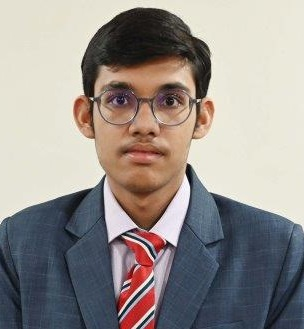
\includegraphics[width=3.0cm,height=1.5cm,keepaspectratio]{m1.png}
\end{minipage}
\\
\hline
\begin{minipage}[t][3.25cm][t]{\linewidth}
\vspace{1.5mm}
\textbf{Team member 2}\\[-1mm]
\textit{}
\vspace{2.0cm}
\end{minipage}
&
\begin{minipage}[t][3.25cm][t]{\linewidth}
\vspace{1.5mm}
\textit{Singh, Bhupendra -- 2510011665}\\
\textit{2510011665@geu.ac.in}

\vspace{2mm}
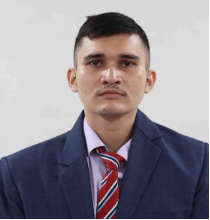
\includegraphics[width=3.0cm,height=1.5cm,keepaspectratio]{m2.png}
\end{minipage}
\\
\hline
\begin{minipage}[t][3.25cm][t]{\linewidth}
\vspace{1.5mm}
\textbf{Team member 3}\\[-1mm]
\textit{}
\vspace{2.0cm}
\end{minipage}
&
\begin{minipage}[t][3.25cm][t]{\linewidth}
\vspace{1.5mm}
\textit{Varshney,Raghav--2510011388}\\
\textit{2510011388@geu.ac.in}

\vspace{2mm}
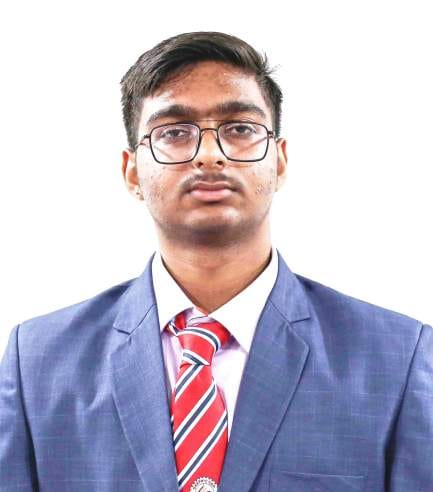
\includegraphics[width=3.0cm,height=1.5cm,keepaspectratio]{m3.png}
\end{minipage}
\\
\hline
\begin{minipage}[t][3.25cm][t]{\linewidth}
\vspace{1.5mm}
\textbf{Team member 4}\\[-1mm]
\textit{}
\vspace{2.0cm}
\end{minipage}
&
\begin{minipage}[t][3.25cm][t]{\linewidth}
\vspace{1.5mm}
\textit{Jakhmola,Ishan --2510012067}\\
\textit{2510012067@geu.ac.in}

\vspace{2mm}
 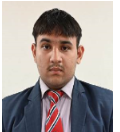
\includegraphics[width=3.0cm,height=1.5cm,keepaspectratio]{m4.png}
\end{minipage}
\\
\hline
\end{tabularx}

\newpage
% ============================================================
% PAGE 2
% ============================================================

\vspace*{0.15cm}

\noindent
\colorbox{GEUBannerBlue}{%
\parbox{\dimexpr\textwidth-2\fboxsep\relax}{
    \vspace{0.18cm}
    {\color{GEUYellow}
    \fontsize{17}{21}\selectfont
    \bfseries
    PHASE-II PROJECT PROGRESS DESCRIPTION }
    \vspace{0.18cm}
}}

\vspace{0.70cm}

% PROJECT ABSTRACT
\sectiontitle{Project Abstract }

\vspace{0.05cm}

\instruction{

}

\vspace{0.12cm}

\answerbox{6.0cm}{Logistics and Delivery Management System is a desktop application that helps users perform logistics and delivery management operations in an efficient manner. This system acts as a medium for managing customer management, deliveries, delivery people management, vehicles, shipments, and delivery status.
The main purpose of the system is to minimize manual effort and organize the whole process of tracking and managing the deliveries. The users will be able to update shipments, assign deliveries, manage delivery people and vehicles, and track the current status of shipments using an interactive graphical user interface.
The development of the application involves C++ and Qt and is implemented from an object-oriented perspective. Various modules are represented in the form of classes in order to increase the flexibility and reusability of the code. Data structures and relevant validation methods are used in the system.
The final system is expected to provide a user-friendly interface that would allow users to get necessary logistics information and perform delivery management operations.}

\vspace{0.70cm}

% UPDATED PROJECT APPROACH
\sectiontitle{Updated Project Approach and Architecture }

\vspace{0.05cm}

\instruction{

}

\vspace{0.25cm}

\answerbox{6.75cm}{• The Logistics and Delivery Management System is being developed as a desktop-based application using C++ and the Qt framework. The project follows a modular, object-oriented architecture that separates the graphical user interface, application logic, and data management. The Qt interface includes a dashboard, forms, tables, and navigation options for managing customers, shipments, delivery personnel, vehicles, and delivery status. C++ classes are designed to represent these entities and handle their respective operations, making the application organized, reusable, and easier to maintain.


• The application uses Qt widgets to create an interactive and user-friendly interface. Qt's signals and slots mechanism connects user actions, such as button clicks and form submissions, to the corresponding functions. Object-oriented concepts, including encapsulation, abstraction, inheritance, and polymorphism, are applied wherever appropriate to improve code structure and reusability. The application also includes input validation and error handling to prevent incorrect data entry. Development is carried out module by module, followed by integration and functional testing to verify that customer management, shipment handling, vehicle assignment, and delivery tracking work together correctly. The main focus is to develop a reliable, efficient, and easy-to-use system that simplifies logistics operations and improves delivery management.}

\newpage

% ============================================================
% PAGE 3
% ============================================================



% TASKS COMPLETED
\sectiontitle{Tasks Completed}

\vspace{0.05cm}

\begin{tabularx}{\textwidth}{
|>{\raggedright\arraybackslash}X
|>{\raggedright\arraybackslash}X|
}
\hline
\textbf{Task Completed} & \textbf{Team Member}\\
\hline

Completed the user, customer, and authentication modules, along with searching, sorting, and binary search algorithms.
&
Kush Agarwal\\
\hline

Completed the delivery, driver, and logistics modules, along with queue and priority queue implementation.
&
Bhupendra Singh Thapa\\
\hline

Completed file handling and validation modules, along with linked list and stack implementation.
&
Raghav Varshney\\
\hline

Developed the Qt-based GUI with a main window, dashboard, widgets, and navigation features.
&
Ishan Jakhmola\\
\hline

\end{tabularx}

\vspace{0.65cm}

% CHALLENGES
\sectiontitle{Challenges/Roadblocks }

\vspace{0.05cm}

\instruction{

}

\vspace{0.18cm}

\answerbox{6.05cm}{Development has presented a number of major problems, not least in the form of the complexity inherent to the different backend modules. This covers everything from data structures and authentication to the management of customers and deliveries. The plan is to put an end to this by breaking the project down into its constituent modules and assigning tasks on an individual basis.

Then there is the matter of the Qt-based graphical user interface and how it is to be integrated with the backend. It is no easy task to ensure that what is done in the UI is relayed correctly to the backend classes; we will address this by way of Qt signals and slots to link the UI components to the right functions.

Consistency of information is also a concern, especially with logistics, so file handling will see some improvement in the code along with the addition of sound error handling and input validation.

As for the team, one can expect integration issues to arise when combining the code they have written. To prevent this, there will be regular communication and a good deal of testing to go along with the distribution of work. In the same vein, both integration and module-level testing will be ongoing.}

\vspace{0.65cm}


% TASKS PENDING
\sectiontitle{Tasks Pending}

\vspace{0.50cm}

\begin{tabularx}{\textwidth}{
|>{\raggedright\arraybackslash}X
|>{\raggedright\arraybackslash}p{0.35\textwidth}|
}
\hline
\textbf{Pending Task} & \textbf{Assigned To} \\
\hline

Feature Development &
Kush Agarwal, Bhupendra Singh Thapa \\
\hline

Module Integration &
Ishan Jakhmola, Bhupendra Singh Thapa \\
\hline

Input Validation &
Raghav Varshney \\
\hline

Error Handling &
Raghav Varshney, Kush Agarwal \\
\hline

Testing and Debugging &
All Team Members \\
\hline

Project Documentation &
All Team Members \\
\hline

\end{tabularx}

% ============================================================
% PAGE 4
% ============================================================

\vspace*{0.30cm}
\newpage
% PROJECT OUTCOME
\sectiontitle{Project Outcome/Deliverables }

\vspace{0.05cm}

\instruction{

}

\vspace{0.35cm}

\answerbox{5.35cm}{At present the project is in the development and integration phase, with a basic architecture in place. To make for easier collaboration and a smoother process, the backend modules have been decoupled.

Some of these are already complete, namely the AuthManager and Customer modules. The rest of the backend consists of the User, Delivery, Driver, LogisticsSystem, FileManager and Validator modules, not to mention the data structures and algorithms required to handle information processing.

On the front end, a graphical interface has been put together with the Qt framework; it is being built on its own and includes the window, dashboard, widgets and means of navigation. What remains is to see the development of the connecting modules through to completion so as to link the GUI with the backend, then test the principal functionality and put right any errors that turn up.}

\vspace{0.75cm}

% PROGRESS OVERVIEW
\sectiontitle{Progress Overview }

\vspace{0.05cm}

\instruction{
}

\vspace{0.25cm}

\answerbox{5.45cm}{- The project is currently at the development and integration stage.

- The fundamental components of the project have been developed, and the backend has been divided into modules to simplify development and interaction.

- The AuthManager and Customer modules have already been implemented.

- The remaining backend modules include User, Delivery, Driver, LogisticsSystem, FileManager, and Validator, along with the algorithms and data structures required for processing and storing information.

- The graphical user interface (GUI), developed using the Qt framework, includes a window, dashboard, widgets, and navigation tools. It is being developed separately from the backend.

- The remaining tasks involve completing the modules that connect the GUI with the backend, testing the main features of the application, and fixing the identified bugs.}


% ============================================================
% PAGE 5
% ============================================================

\vspace*{0.20cm}




% CODEBASE INFORMATION
\sectiontitle{Codebase Information}

\vspace{0.55cm}

\begin{tabularx}{\textwidth}{
|>{\raggedright\arraybackslash}p{0.30\textwidth}
|>{\raggedright\arraybackslash}X|
}
\hline
\textbf{Category} & \textbf{Description} \\
\hline

Repository Link &
\url{https://github.com/agarwkush/PBL} \\
\hline

Codebase Overview &
The GitHub repository contains the project's source code and related files. It helps the team organize code, track changes, collaborate on development, and maintain project updates. \\
\hline

\end{tabularx}


\vspace{0.25cm}

% TESTING
\sectiontitle{Testing and Validation Status}

\vspace{0.05cm}

\instruction{}

\vspace{0.30cm}

\begin{tabularx}{\textwidth}{
|>{\raggedright\arraybackslash}p{0.34\textwidth}
|>{\raggedright\arraybackslash}p{0.20\textwidth}
|>{\raggedright\arraybackslash}X|
}
\hline

\textbf{Module Tested} &
\textbf{Result} &
\textbf{Remarks}
\\
\hline

User Authentication &
Pass &
Valid credentials verified.
\\
\hline

Customer Data Management &
Pass &
Customer records managed successfully.
\\
\hline

Driver Allocation and Delivery Tracking &
Pass &
Driver assignment and status updates verified.
\\
\hline

File Handling &
Pass &
File read and write operations verified.
\\
\hline

Data Structure Implementation &
In Progress &
Testing data structure operations.
\\
\hline

Searching and Sorting Algorithms &
In Progress &
Verifying search and sorting accuracy.
\\
\hline

Input Validation and Error Handling &
Pass &
Invalid inputs handled correctly.
\\
\hline

Qt GUI Integration &
In Progress &
Testing GUI and backend integration.
\\
\hline

\end{tabularx}

\vspace{0.65cm}
\newpage
% DELIVERABLES PROGRESS
\sectiontitle{Deliverables Progress }

\vspace{0.05cm}

\instruction{

}

\vspace{0.25cm}

\answerbox{5.20cm}{-Project Planning: Identified the key requirements for the Logistics and Delivery Management System.

- UI Design: Developed the first draft of the app interface with Qt.

Module Design: Designed the core modules for delivery, shipping information, and logistics.

- System Architecture: Defined the basic architecture of the application and how the different parts interact.

- Implementation Progress: Initiated structuring of the source code and development of the application’s initial components.

- Project Status: The project is in development status and further implementation is ongoing.

- Work to be done: Development of core functionality, integration of modules, testing, error fixing and documentation preparation.}
\end{document}